\section{Results and Discussion}

Euclidian coordinates performed better when speaking of efficiency in terms of accuracy and speed. 76.92\% of the Euclidian charts shown resulted in the a correct identification of the real data while only 20.31\% of the polar charts did the same. A t-test comparing means for charts with polar coordinates versus charts with Euclidian coordinates resulted in a t statistic of 15.2013 with a p-value of 2.2e-16. Similarly, a t-test comparing means of time spent on charts with Euclidian coordinates versus charts with polar coordinates resulted in a p-value of 1.014e-11. The average of the log of time spent on each individual chart for charts with Euclidian coordinates is 3.53 minutes while it was 4.07 minutes for charts with polar coordinates. Euclidian coordinates resulted in a significantly more accurate identification of the real data set in significantly shorter time. 

\begin{figure}[htbp] %  figure placement: here, top, bottom, or page
   \centering
   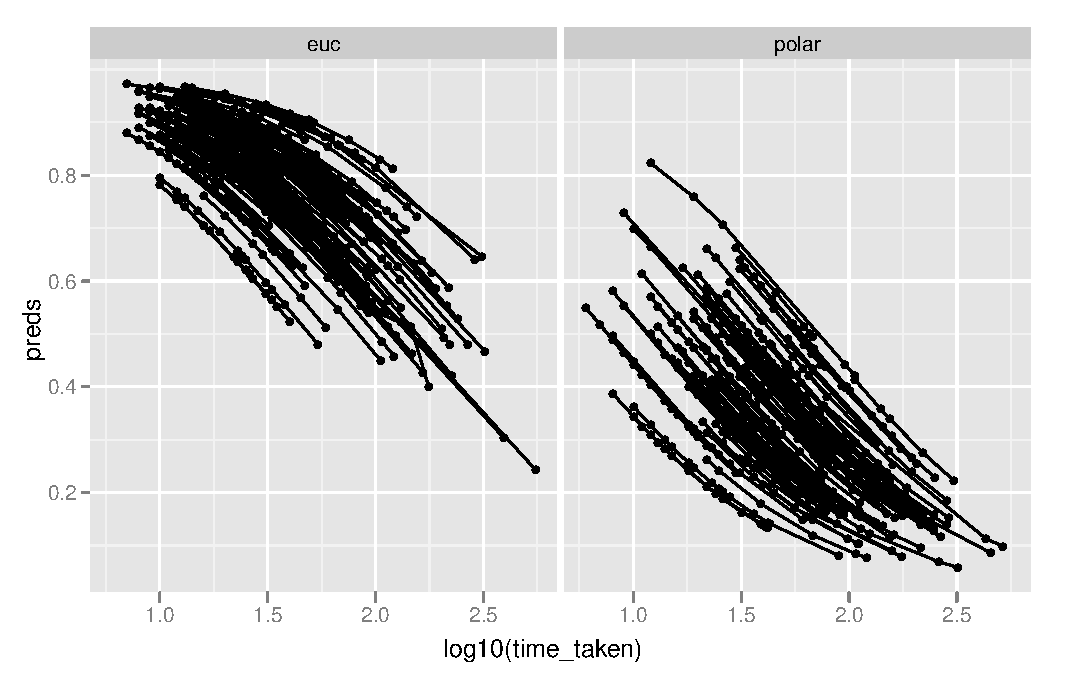
\includegraphics[width=3in]{turk4_time_perc_preds.pdf}  
   \caption{Values predicted from XXXX how to say itXXXX of accuracy for log of time taken and test parameter.}
   \label{accuracy_preds}
\end{figure}

Figure \ref{accuracy_preds} shows predicted accuracy levels. These predicted values were obtained by using R package lme4 and a mixed effect model explaining correct responses by type of chart and the log of time spent while accounting for different levels of accuracy for each individual who participated in the experiment. The predicted values show that there is an overall higher accuracy level for Euclidian coordinates when compared to polar coordinates. For both chart types, as the time spent increases, the predicted accuracy decreases. 

\begin{figure}[htbp] %  figure placement: here, top, bottom, or page
   \centering
   %\includegraphics[width=3in]{turk4_samplesize_correctn.pdf}  
   \caption{For each sample size for polar and Euclidian coordinates, the bars are colored according to the number of correct responses. Darker colors indicate lower accuracy levels while lighter colors indicate higher accuracy levels. }
   \label{samp_size_acc}
\end{figure}

Ideally, efficient detection of data characteristics will be possible at small sample sizes. The difficulty of the charts is largely determined by the sample size taken from the original data set. Samples of 24 \% generally result in higher accuracy as the extra information facilitates detection of a relationship. Figure \ref{accuracy_preds} shows the relationship between the number of correct responses relative to the total number of responses and how this relationship differs between Euclidian and polar coordinates. The bars in the Euclidian plot are overall a lighter color than they are in the polar plot. This indicates a higher level of accuracy at all sample sizes. For Euclidian coordinates, we can see a stair step pattern in the accuracy levels as sample size increases. Lower levels of accuracy, indicated by darker colors, become consistently less prevelant as sample size increases. The relationship between sample size and accuracy level is not as simple for polar coordinates. Sample sizes of 2\% and 4\% have very similar accuracy levels. After 6\% the stair step pattern becomes visible and similar to that of Euclidian coordinates. Sample size seems to have less of an effect on accuracy for polar coordinates than it does for Euclidian coordinates. Predicted values of the proportion of correct responses when explained by sample size, the type of chart, and the interaction between these two factors, show that there is a significant difference between the relationship between sample size and correct responses for polar and euclidian coordinates. Indeed, the proportion of correct responses increases more rapidly as sample size increases for Euclidian coordinates than it does for polar coordinates. 

The effect of a reference line on accuracy and time was not statistically significant for both types of charts. When looking at plots of the data, however, the time spent on the charts seems to be higher when there is a reference line.This is true for both Euclidian and polar charts. Also visible in the data is a slight increase in accuracy with the presence of a reference line. These characteristics can be seen in figure\ref{reflines}.  

\begin{figure}[htbp] %  figure placement: here, top, bottom, or page
   \centering
   \includegraphics[width=2in]{turk4_refilne_time.pdf}  
   \includegraphics[width=2in]{turk4_refline_correctn.pdf}  
   \caption{The relationship between reference line and time spent (left) and the relationship between reference line and accuracy (right). Although not statistically significant, some patterns are visible.}
   \label{reflines}
\end{figure}







